\Chapter{Folyamatelemzés}

A dolgozatban ismertetésre kerül két folyamatelemzési algoritmus, melyek célja, illetve számos paramétere átfedésben van. Ezeknek a célja, hogy eseménysorozatok halmazá\hyp{}ból egy ok-okozat rendszert építsen fel.

A működésükben az eseménysorok halmazát nevezhetjük eseménynaplónak is. Ez az eseménynapló úgynevezett trace halmazoknak a halmaza, egy trace pedig adott tevékenységnek a sorozata. Ezen fogalmak formális bevezetését láthatjuk a továbbiak\hyp{}ban.

\subsection{Eseménynapló}
Az eseménynapló az elsődleges szükséglet bármely folyamatbányászati algoritmus alkal\hyp{}mazásához.

Az eseménynapló a következőket tartalmazza: egyedi azonosító az esethez, tevékeny\hyp{}ség megnevezése valamint egy időbélyeg. Egy eseménynaplót akár tevékenységek halma\hyp{}zának halmazaként is lehet ábrázolni.

\begin{definition}{\textit{(Munkafolyamati trace)}} Egy sztring a $T$ ábécé feladatai közül.\end{definition}
\begin{definition}{\textit{(Munkafolyamati napló)}} Munkafolyamati tracek halmaza.\end{definition}

Számos gyakorlati megvalósításban a munkafolyamati naplót a munkafolyamattól függően át kell formázni, hogy egyértelműen tartalmazza a szükséges adatokat, majd az így kapott eredményt nevezzük eseménynaplónak.

\Section{Alpha-algoritmus}

Az Alpha-bányász volt a legelső folyamatbányászati módszer amit javasoltak és egy egész jó rálátást biztosít a folyamatbányászat céljára, valamint arra, hogy a folyamatok\hyp{}ban lévő különböző tevékenységek hogyan is hajtódnak végre. Emelett, az Alpha\hyp{}bányász szolgált számos újabb folyamatbányászati technika (pl.: Heurisztikus bányász, genetikus bányászat) alapjaként. Először van der Aalst, Weijters és Măruşter hozta be a köztudatba. 

Az algoritmus egy munkafolyamati naplót $W \subseteq  T^*$ kap bemenetként, és eredmény\hyp{}ként egy munkafolyamati hálót épít fel.

Ezt az alapján csinálja meg, hogy megvizsgálja az általános kapcsolatokat az egyes feladatok között. Például egy adott feladat lehet, hogy minden esetben megelőz egy másik feladatot, ami egy hasznos információ.

Az Alpha-bányász szabályai szerint az egyes tevékenységek között az alábbi 4 féle kapcsolat egyike lehetséges.
\begin{enumerate}
\item \textbf{Közvetlen sorrend: $x > y$} akkor és csakis akkor ha az $x$ eseményt közvetlenül követi $y$.
\item \textbf{Okozat: $x \rightarrow y$} ha $x > y$ és nem $y > x$.
\item \textbf{Párhuzam: $x \parallel y$} ha $x > y$ és $y > x$.
\item \textbf{Választás: $x \# y$} ha nem $(x > y)$ és nem $(y > x)$.
\end{enumerate}

\subsection{Grafikus ábrázolás}

\vfill

\begin{figure}[h!]
\begin{center}

\includegraphics[width=0.5\textwidth,keepaspectratio=true]{images/img_alpha_seq}\\
\caption{\textbf{Szekvencia: A $\rightarrow$ B}}
\label{fig:example}
\end{center}
\end{figure}

\vfill

\begin{figure}[h!]
\begin{center}
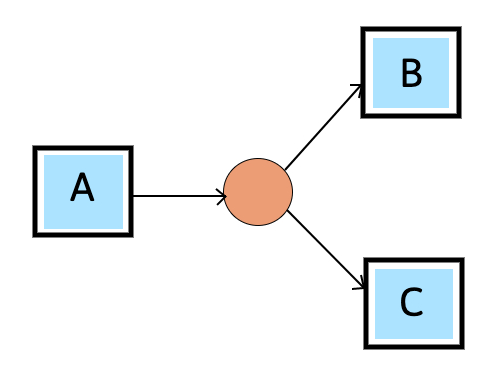
\includegraphics[width=0.5\textwidth,keepaspectratio=true]{images/img_alpha_xor}\\
\caption{\textbf{XOR-elágazás: A $\rightarrow$ B, A $\rightarrow$ C} és \textbf{B \# C}}
\label{fig:example}
\end{center}
\end{figure}

\vfill

\begin{figure}[h!]
\begin{center}
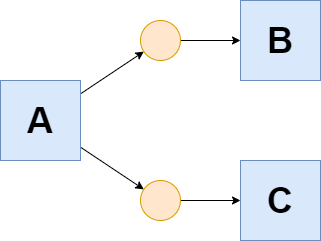
\includegraphics[width=0.5\textwidth,keepaspectratio=true]{images/img_alpha_and}\\
\caption{\textbf{ÉS-elágazás: A $\rightarrow$ B, A $\rightarrow$ C} és \textbf{B $\parallel$ C}}
\label{fig:example}
\end{center}
\end{figure}

\newpage

\subsection{Példa}
Vegyük példának a 2.1. táblázatban látható eseménynaplót.\\
\begin{table}[h]
\begin{center}
\caption{Példa eseménynapló}
\begin{tabular}{||c | c | c ||}
	\hline
	ID & Tevékenység & Időbélyeg \\ [0.5ex]
	\hline\hline
	1 & A & 2022-10-05 13:50:40.000 \\
	\hline
	1 & B & 2022-10-05 16:30:12.000 \\
	\hline
	1 & C & 2022-10-05 16:57:31.000 \\
	\hline
	1 & D & 2022-10-06 13:50:41.000 \\
	\hline
	2 & A & 2022-10-06 15:30:27.000 \\
	\hline
	2 & C & 2022-10-06 16:23:33.000 \\
	\hline
	2 & B & 2022-10-07 08:33:02.000 \\
	\hline
	2 & D & 2022-10-07 12:41:11.000 \\
	\hline
	3 & A & 2022-10-07 13:02:57.000 \\
	\hline
	3 & E & 2022-10-07 14:11:21.000 \\
	\hline
	3 & D & 2022-10-07 14:59:22.000 \\
	\hline
\end{tabular}
\label{fig:example}
\end{center}
\end{table}\\	
Ebben az esetben az eseménynaplót az alábbi módon tudjuk jelölni:
\[ 
	L_1 = [< A,B,C,D >, <A,C,B,D>, <A,E,D>].
\]

Az Alpha-bányász úgy kezdi a munkát, hogy az eseménynaplót közvetlen-sorrend, okozat, párhuzam és választás relációkra alakítja, és ezeket felhasználva létrehoz egy Petri-hálót, ami leírja a folyamat modelljét.

Első lépésként létrehoz egy lenyomati mátrixot.

\begin{table}[h!]
\begin{center}
\caption{Példa lenyomati mátrix}
\begin{tabular}{|c | c | c | c | c | c|}
	\hline
	\hspace{0.1cm} & A & B & C & D & E \\
	\hline
	A & \# & $\rightarrow$ & $\rightarrow$ & \# & $\rightarrow$ \\
	\hline
	B & $\leftarrow$ & \# & $\parallel$ & $\rightarrow$ & \# \\
	\hline
	C & $\leftarrow$ & $\parallel$ & \# & $\rightarrow$ & \# \\
	\hline
	D  & \# & $\leftarrow$ & $\leftarrow$ & \# & $\leftarrow$ \\
	\hline
	E & $\leftarrow$ & \# & \# & $\rightarrow$ & \# \\
	\hline
\end{tabular}
\label{fig:example}
\end{center}
\end{table}

\newpage

\noindent $Y_W$ az összes $(A,B)$  pár halmaza a feladatok maximális halmazából úgy, hogy:
\begin{itemize}
	\item {egyik $A \times A$ és $B \times B$ sem tagja $>$-nek, és}
	\item {$A \times B$ részhalmaza $\rightarrow$-nek.}
\end{itemize}
\noindent $P_W$ tartalmazza az egyes $Y_W$-hez tartozó helyeket $p_{(A,B)}$, plusz a beviteli $i_W$ helyet és a kimeneti $o_W$ helyet.
\noindent A folyamati reláció $F_W$ az alábbiak uniójából áll össze:
\begin{itemize}
\item $\{(a,p_{(C,B)})|(A,B) \in Y_W \wedge a \in A\}$,
\item $\{(p_{(A,B)},b)|(A,B) \in Y_W \wedge b \in B\}$,
\item $\{(i_W,t)|t \in T_1\}$,
\item $\{(t,i_0)|t \in T_0\}$.
\end{itemize}

\noindent Az eredmény

\begin{itemize}
\item egy Petri-háló struktúra $\alpha (W) = (P_W, T_W, F_W)$,
\item egy beviteli hellyel $i_W$ és egy kimeneti hellyel $o_W$.
\item Mivel minden $T_W$ átmenet $F_W$-úton van $i_W$-ből $o_W$-be, így valóban egy munka\hyp{}folyamati háló.
\end{itemize}

\noindent Ehhez a példához 2.4 ábrán látható Petri-háló jön létre az Alpha-bányász használatával.
\begin{figure}[h]
\begin{center}
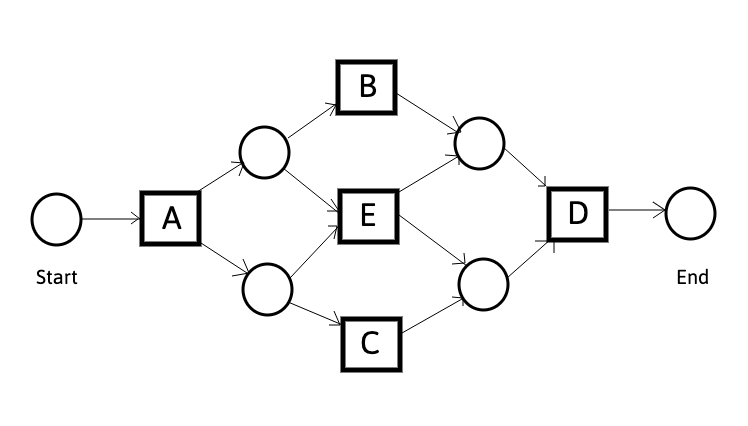
\includegraphics[width=\textwidth,height=\textheight,keepaspectratio]{images/img_alpha_petri_output}\\
\label{fig:example}
\end{center}
\caption{Példa kimeneti Petri-háló}
\end{figure}

\newpage

\subsection{Korlátozások}
\begin{itemize}
\item \textbf{Implicit helyek}: Az Alpha-bányász nem tud különbséget tenni az implicit és a szükséges helyek között, így a felfedezett Petri-hálóban előfordulhatnak plusz szükségetelen helyek.
\item \textbf{Ciklusok}: Az Alpha-bányász nem képes 1-es és 2-es hosszúságú ciklusok felisme\hyp{}résére a folyamatmodellben.
\item A helyi függőségeket gyakran nem veszi észre az Alpha-bányász.
\end{itemize}
\cite{1316839}

\Section{Heurisztikus Bányász}

Az Alpha-algoritmushoz hasonlóan ez is egy folyamatbányászati technika, mely lehetőve teszi eseménynaplókból információ kinyerését.

Ennek a sikerességéhez, az események sorrendjét csupán az egyes esetekben veszi figyelembe, azaz nem számít a sorrendjük esetek között.

\subsection{Működése}

Ahhoz, hogy egy folyamatmodellt meg lehessen találni egy eseménynapló alapján, azt elemezni szükséges. Találni kell okozati függőséget, például ha egy tevékenységet mindig követ egy másik adott tevékenység, akkor nagy valószínűséggel feltételezhető, hogy függőségi reláció van közöttük. 

Ezeknek a relációknak az elemzéséhez vegyük az alábbiakat:

\begin{definition}{\textit{(Heurisztikus bányász):}} Legyen $W$ egy eseménynapló adott $T$ felett, azaz $W \subseteq T^*$. Emellett legyen $a,b \in T:$
\begin{enumerate}

\item $ a>_W b $, ha létezeik $\sigma = t_1 t_2 t_3 \ldots t_n $ trace és $i \in \{1, \ldots ,n-1\}$ úgy, hogy $\sigma \in W$ és $t_i=a$, valamint $t_{i+1}=b$,
\item $ a \rightarrow_W b $, ha $a>_W b$ és $b\ngtr_W a$, 
\item $ a\#_Wb $, ha $a \ngtr_W b$ és $b\ngtr_W a$,
\item $a\parallel_Wb $, ha $a>_W b$ és $b>_Wa$,
\item $a >>_Wb$, ha létezik $\sigma = t_1 t_2 t_3 \ldots t_n $ trace és $i \in \{1, \ldots ,n-2\}$ úgy, hogy $\sigma \in W$ és $t_i=a$, $t_{i+1}=b$ és $t_{i+2}=a$,
\item $a>>>_Wb$, ha létezik $\sigma = t_1 t_2 t_3 \ldots t_n $ trace, $i<j$ és $i,j \in \{1,\ldots,n\}$ úgy, hogy $\sigma \in W$ és $t_i=a$, $t_j=b$.

\end{enumerate}
\end{definition}

\subsection{Lépései}

\subsubsection{Első lépés: a függőségi gráf bányászata}

 A Heurisztikus Bányász első lépése az úgynevezett \textit{függőségi gráf} felépítése. Ez egy gyakoriság alapú rendszer, mely azt mutatja meg, hogy mennyire lehetünk biztosak abban, hogy valóban létezeik függőségi reláció az egyes események között.

A kiszámított értékeket arra lehet használni egy heurisztikus keresésben, hogy megkapjuk a helyes függőségi relációt.

Legyen $W$ egy eseménynapló adott $T$ felett, valamint $a,b \in T$. Ekkor $|a>_W b|$ annak a száma, hogy $a>_Wb$ mennyiszer fordul elő $W$-ben és az
\[
a \Rightarrow_W b = \left(\frac{|a>_Wb|-|b>_Wa|}{|a>_Wb|+|b>_Wa|+1}\right)
\]
arány a függőség erősségét jelzi. Fontos megjegyezni, hogy ez alapján $a\Rightarrow_Wb$ értéke mindig -1 és 1 között van. Egy magas érték alapján erősen feltételezhető, hogy létezik a függőségi relacíó.

\subsubsection{Második lépés: a ciklusok felismerése}

Egy folyamatban előfordulhat, hogy egy adott tevékenység többször kerül végrehajtás\hyp{}ra. Ez tipikusan ciklusnak felel meg az adott modellben.

A távoli ciklusok (pl.: ...\textit{ABCABCABC}...) nem jelentenek problémát a Heurisztikus bányásznak, azonban az egyes hosszúságú (pl.: \textit{ACB, ACCB, ACCCB}, ... tracekben) és kettes hosszúságú (pl. olyan tracek mint: \textit{ACDB, ACDCDB, ACDCDCDB}) ciklusoknál a $C\Rightarrow_WC$ és $C\Rightarrow_WD$ értéke mindig nagyon alacsony.

Szerencsére nagyon egyszerű módon lehet definiálni a függőség mértékét ezekre a ciklusokra. Legyen $W$ egy eseménynapló adott $T$ felett, valamint $a,b \in T$. Ekkor $|a>_W b|$ annak a száma, hogy $a>_Wb$ mennyiszer fordul elő $W$-ben, illetve $|a>>_Wa|$ annak a száma, hogy $a>>_Wb$ mennyiszer fordul elő W-ben, ahol
\[
a\Rightarrow_Wa=\left(\frac{|a>_Wa|}{|a>_Wa|+1}\right),
\]
\[
a\Rightarrow_{2\ W} b=\left(\frac{|a>>_Wb|+|b>>_Wa|}{|a>>_Wb|+|b>>_Wa|+1}\right).
\]

\subsubsection{Harmadik lépés: a távoli függőségek feltérképezése}

Néhány folamatmodellben, két tevékenység közül történő választás nem feltétlenül egy adott lépésben dől el, hanem a folyamatmodell más részein történő választásoktól függhet.

\begin{figure}[h!]
\begin{center}
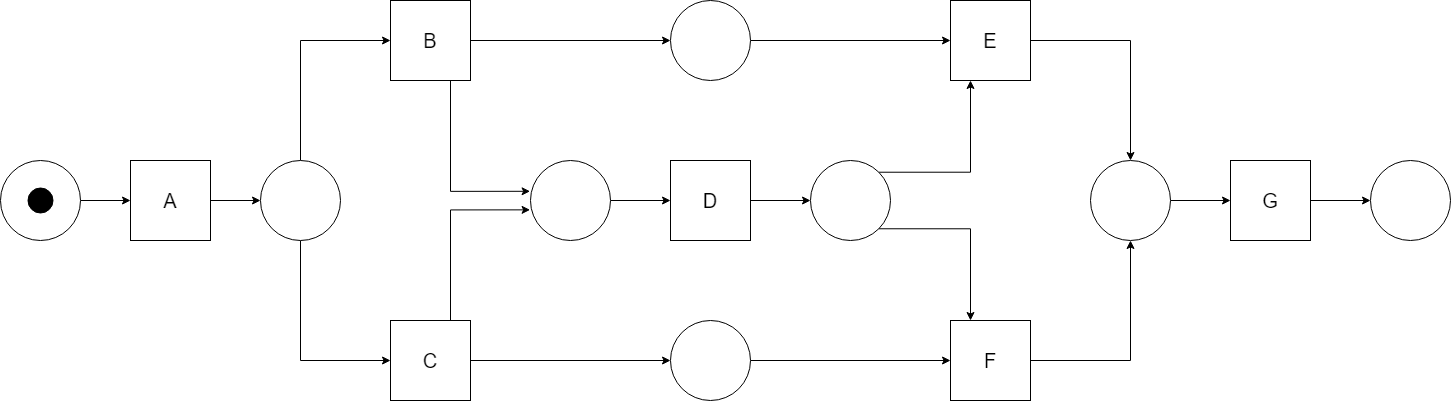
\includegraphics[width=\textwidth,keepaspectratio=true]{images/img_heuristic_longdistance}
\label{fig:plan}
\end{center}
\caption{Folyamatmodell távoli függőséggel}
\end{figure}

A 2.5-ös ábrán látható egy távoli függőség felépítése. \textit{D} tevékenység végrehajtása után \textit{E} és \textit{F} tevékenységek közül lehet választani. Azonban ezt az \textit{E} és \textit{F} közötti választást egy korábbi, \textit{B} és \textit{C} közüli választás előzi meg. Egyértelműen, ezeket a nem-lokális viselkedéseket kifejezetten nehéz bányászni az olyan megközelítésekkel melyek bináris információ alapján ($a>_Wb$) működnek. Csupán néhány algoritmus képes sikeresen bányászni őket.

Azt az eseménynaplót amelyet a 2.5-ös ábra folyamatmodellje alapján kapunk, a Heurisztikus Bányász eddig bemutatott állapotában úgy fogja elemezni, hogy a függőségi gráfban nem fog szerepelni a $B\rightarrow E$ és $C\rightarrow F$ kapcsolat. Azonban az említett $a>>>_Wb$ reláció erősen jelezni fogja, hogy \textit{B}-t mindig követi \textit{E}, \textit{C}-t pedig \textit{F}. Például ha |\textit{B}| a gyakorisága \textit{B}-nek, akkor $B\Rightarrow_W^l E = |B >>>_WE|/|B|+1$ értéke 1-hez közeli lesz, azonban sok magas $\Rightarrow_W^l $ érték már összhangban van a folyamatmodellel. Ennek megfelelően, a 2.5-ös ábra alapján az $A\Rightarrow_W^lD$ értéke közel lesz 1-hez, viszont nincsen szükség a plusz függőségi relációra.

Ezt az alapján lehet ellenőrizni, hogy az eddig bányászott folyamatmodellen letesz\hyp{}teljük, hogy lehetséges-e \textit{A}-ból a végállapotba (\textit{G}) eljutni anélkül, hogy áthalad\hyp{}nánk \textit{D} tevékenységen. Csakis akkor, ha ez lehetséges, akkor kerül a folyamatmodell frissítésre az extra \textit{A}-ból \textit{D}-be függőségi relációval.
\cite{book:heuristic}

\Section{Robotic Process Automation} 

A Robotikus Folyamatautomatizálás (továbbiakban: RPA) egy olyan szoftvertechnoló\hyp{}gia, mely lehetővé teszi, hogy az erre specializált szoftverek emberi felhasználót emulál\hyp{}va lépjenek kapcsolatba a számítógépek digitális felületeivel.

Minden egyes ilyen szoftvernek más az eszköztára, van amelyik azt tudja értelmezni, hogy mi van a képernyőn, van amelyik felismer és kinyer adatokat, viszont abban mindegyik osztozik, hogy adott lépésekből meghatározott folyamatokat hajt végre.

Összefoglalva, egy ilyen tökéletesített rendszer ugyanazt tudja, mint egy felhasználó, viszont sokkal gyorsabban és konzisztensebben, anélkül, hogy fel kellene állnia nyújtózni vagy elmenni egy kávészünetre.

\subsection{Alkalmazási területek}

Lényegében bármely olyan modern cég tudja hasznosítani ezt a technológiát, mely számítógépet használva például nyilvántartást vezet, pénzügyeit digitálisan kezeli, alap\hyp{}vetően a digitális térben mozog, tehát bárhol, ahol embereket digitális tevékenységük alól fel lehet szabadítani.

Elsősorban az adott cégtől függ, hogy belevág-e egy ilyen szoftvertechnológiás meg\hyp{}oldásba, a következőkben szerepel néhány szektor ahol alkalmazható, vagy már alkalma\hyp{}zásra is került:
\begin{itemize}
	\item Egészségügy,
	\item Telekommunikáció,
	\item Gyártástechnológia,
	\item Állami szektor,
	\item Kereskedelem,
	\item Pénzügyi szolgáltatások.
\end{itemize}

Gyakorlatilag csupán az adott folyamattól függ, hogy lebontható-e olyan triviális lépésekre, melyeket már az RPA eszközkészletével automatizálni lehet. Természetesen, ahogy fejlődik ez a technológia, úgy egyre nagyobb százalékban lehet majd ezeket is automatizáltnak tekinteni.

Alább található néhány mai rendszer, melyeket a technológia úttörőjének lehet nevezni:
\begin{itemize}
	\item UIPath\cite{rpa:uipath},
	\item Microsoft Power Automate\cite{rpa:microsoftpowerautomate},
	\item Blue Prism\cite{rpa:blueprism},
	\item Automaton Anywhere\cite{rpa:automationanywhere},
	\item Kofax\cite{rpa:kofax}.
\end{itemize}

\Section{Delphi}

A dolgozathoz készült szoftver Delphi nyelven íródott, így fontos legalább nagyvona\hyp{}lakban ismerni a nyelvet, hogy megértsük a választás okát.
A Delphi egy általános célú, erősen típusos, objektum orientált programozási nyelv és szoftvertermék, ami az Object Pascal programozási nyelv Delphi dialektusát használ\hyp{}ja, integrált fejlesztői környezetet biztosít, újabban a gyors alkalmazásfejlesztés (RAD, Rapid Application Development) szoftverfejlesztési elv szerint. A Delphi fordítói natív kódot generálnak a célrendszertől függően, legyen az Microsoft Windows, macOS, iOS, Android vagy Linux (x64).\textit{\cite{delphi:001}}

\subsection{Múltja röviden}
Az ,,anyanyelve" a Delphinek a Pascal, ami pedig a modellje nagy részét az Algolnak köszönheti -- az első magasszintű progamozási nyelvnek ami olvasható, struktúrált és szisztematikusan meghatározott szintaxissal rendelkezik. A hatvanas években számos utódját fejlesztették az Algolnak, ezek közül a legsikeresebb a Pascal volt.

1983-ban jelent meg az első Turbo Pascal a Borland jóvoltából, ami már integrált fejlesztői környezettel rendelkezett. 1995-ben vezették be a RAD szoftverfejlesztési elvre épülő környezetet, amit Delphi-nek neveztek, ezáltal átalakítva a Pascal nyelvet egy objektum-orientált vizuális programozási nyelvvé. A célja ennek elsősorban az volt, hogy ennek az új terméknek központi részét képezzék az adatbázis eszközök és kapcsolatok.

2006-ban a Borland átadta a fejlesztőeszközöket a CodeGear nevű leányvállalatá\hyp{}nak, majd ezt a leányvállalatot 2008-ban eladta az Embarcadero Technologies-nek. Ez az új cég megtartotta a régi fejlesztői divíziót és számos új verziót dobott piacra. 2015-ben az Idera Software nevű cég pedig felvásárolta az Embarcadero-t és mind a mai napig ugyanúgy Embaracadero márka alatt működteti a fejlesztői eszközök divízióját.

Az évek alatt rendkívül sok modernizáción ment át a Delphi. OLE (Object Linking and Embedding) automatizáció és változó adattípus támogatásától kezdve, DLL debu\hyp{}goláson és XML támogatáson keresztül egészen a multi-platform alkalmazásokig és az in-line változó deklarálásig.\textit{\cite{delphi:002}}

\subsection{Napjainkban}

Sajnos számos rosszul időzített és rosszul kivitelezett marketing döntés miatt a 2000-es évektől kezdve a Delphi kifejezetten kiesett rengeteg programozó kedvelt programozási nyelve közül, azonban az elmúlt néhány évben ismét sikerült egyre nagyobb ismertségre szert tennie a komolyabb fejlesztők körében.

Bár közel sem a legelterjedtebb nyelv, számos előnnyel rendelkezik sok másikkal szemben. Ilyenek például az alábbiak.
\begin{enumerate}
	\item \textbf{Könnyen olvasható kód}: Már eredetileg a Pascal megalkotásánál az egyik fő cél az volt, hogy oktatási célra lehessen használni, emberi szemmel is könnyen olvasható legyen a komplex alacsony-szintű kód. Erre egy nagyon jó példa a "\{" és "\}" karakterek (amiket csak a memóriával való spórolás miatt jelöltek így) "begin" és "end" kulcsszóra való cseréje.
	\item \textbf{Multi-platformitás}: A megfelelően megírt (OS-független) kódot néhány kattin\hyp{}tással le lehet fordítani a legismertebb operációs rendszerek natív kódjára.
	\item \textbf{Natív kód}: Az alkalmazás lefordításával natív kódot kapunk, ami azért előnyös, mert semmilyen egyéb keretrendszer telepítésére nincsen szüksége (pl.: .NET keretrendszer, Java Runtime Environment)
	\item \textbf{Adatbázis támogatás}: Számos adatbázis kapcsolatot és adatfeldolgozási mód\hyp{}szert beépített módon támogat.
	\item \textbf{Fordítási sebesség}: A mai napig az egyik leggyorsabb a fordítási sebessége más fejlesztőeszközökhöz képest, ezáltal felgyorsítva magát a fejlesztési és hibakeresési folyamatokat.
\end{enumerate}

\subsection{Delphi a dolgozathoz}

Az előző alfejezetben felsoroltaknak megfelelően kiderült, hogy a Delphi az egy kifeje\hyp{}zetten robosztus és erőteljes programozási nyelv. Ez sok nyelvről elmondható természe\hyp{}tesen, viszont az alábbi két pont miatt került kiválasztásra a dolgozathoz.

\begin{itemize}
	\item \textbf{Modern Windows API}: A fejlesztett szoftver (mint a legtöbb RPA eszköz) közvetlen kapcsolatban van a Windows API-val, hiszen az operációs rendszer teszi elérhetővé az egyes erőforrásokat (pl. rögzíteni a felhasználó bevitelét még akkor is, ha a program háttérben van), illetve teszi lehetővé az input injektálását a folyamat visszajátszásához.
	\item \textbf{Natív kód}: Mivel natív kódra kerül fordításra a programkód, ezért bármely Windows (Vista vagy újabb) operációs rendszerrel rendelkező számítógépen fut\hyp{}tatható a program bármiféle keretrendszer nélkül.
\end{itemize}














